\documentclass[12pt]{article}%
\usepackage{amssymb}
\usepackage{amsfonts}
\usepackage{amsmath}
\usepackage[nohead]{geometry}
\usepackage[singlespacing]{setspace}
\usepackage[bottom]{footmisc}
\usepackage{indentfirst}
\usepackage{endnotes}
\usepackage{graphicx}
\usepackage{rotating}
\usepackage{hyperref}
\usepackage{enumitem}

% due to Subfloats section in  
% http://en.wikibooks.org/wiki/LaTeX/Floats,_Figures_and_Captions
\usepackage{graphicx}
\usepackage{caption}
\usepackage{subcaption}

\usepackage{float}

\usepackage{array}
\usepackage{longtable}
\usepackage{fullpage}
\usepackage{dcolumn}
\usepackage[flushleft]{threeparttable}
\usepackage{booktabs}
\usepackage[12hr]{datetime}
\usepackage[DIV=16]{typearea}
\usepackage{scrextend,booktabs}
\usepackage{tabulary}
\usepackage{multirow}
\usepackage[font=footnotesize]{caption}

% due to 
% \usepackage{graphicx}
\usepackage{wrapfig}
\usepackage{lscape}
% \usepackage{rotating}
\usepackage{epstopdf}

\setcounter{MaxMatrixCols}{30}
\newtheorem{theorem}{Theorem}
\newtheorem{acknowledgement}{Acknowledgement}
\newtheorem{algorithm}[theorem]{Algorithm}
\newtheorem{axiom}[theorem]{Axiom}
\newtheorem{case}[theorem]{Case}
\newtheorem{claim}[theorem]{Claim}
\newtheorem{conclusion}[theorem]{Conclusion}
\newtheorem{condition}[theorem]{Condition}
\newtheorem{conjecture}[theorem]{Conjecture}
\newtheorem{corollary}[theorem]{Corollary}
\newtheorem{criterion}[theorem]{Criterion}
\newtheorem{definition}[theorem]{Definition}
\newtheorem{example}[theorem]{Example}
\newtheorem{exercise}[theorem]{Exercise}
\newtheorem{lemma}[theorem]{Lemma}
\newtheorem{notation}[theorem]{Notation}
\newtheorem{problem}[theorem]{Problem}
\newtheorem{proposition}{Proposition}
\newtheorem{remark}[theorem]{Remark}
\newtheorem{solution}[theorem]{Solution}
\newtheorem{summary}[theorem]{Summary}
\newenvironment{proof}[1][Proof]{\noindent\textbf{#1.} }{\ \rule{0.5em}{0.5em}}
\makeatletter
\def\@biblabel#1{\hspace*{-\labelsep}}
\makeatother
\geometry{left=1in,right=1in,top=1.00in,bottom=1.0in}

\begin{document}

\title{Unraveling a secret: Vietnam's outstanding performance on the PISA tests}
\author{Suhas D. Parandekar\thanks{e-mail: \textit{sparandekar@worldbank.org}. This paper has been written using open source software: R for the econometric analysis and graphics and LaTeX for typesetting. Thanks to all who make free software possible and to OECD for making the PISA data freely and easily available to anyone. The code used in writing this paper is freely available for download at \href{http://economist-at-work-and-play.blogspot.com/2015/02/pisa20121a.html}{http://economist-at-work-and-play.blogspot.com/2015/02/pisa20121a.html}}\\Elisabeth K. Sedmik\medskip\\{\normalsize Global Practice for Education, The World Bank} 
\date{\normalsize Date of this draft: \today }}
\maketitle

\sloppy

\singlespacing

\textbf{Abstract}

This paper presents an analyis of the factors that explain Vietnam's outstanding performance on the PISA assessment in 2012. The paper presents a comparative analytical perspective between Vietnam and Colombia, using an Oaxaca-Blinder decomposition of a test score production function. The findings reveal that a) b) and c). 

\strut

\textbf{Keywords:} PISA;Vietnam;Colombia;Oaxaca-Blinder Decomposition; Economics of Education.

\strut

\textbf{JEL Classification Numbers:} I21 (Analysis of Education); I28(Government Policy); Z18(Public Policy).

\thispagestyle{empty}

\pagebreak%
\onehalfspacing
%\doublespacing

\section{Introduction}
Vietnam participated in PISA for the first time in 2012 and its performance has been much higher than other developing countries that take part in this OECD led initiative. PISA scores are calibrated to an OECD mean of 500 and standard deviation of 100 points. Only a few developing countries take part in PISA, perhaps because most of them have results much lower than the OECD countries. As can be seen in Figure 1, there is a positive, albeit non-linear correlation between GDP per capita and PISA test scores that can be seen by the dashed line representing a loess regression. The figure shows that Vietnam's performance in PISA (mathematics mean score of 511) is closer to that of Finland and Switzerland rather than of Peru and Colombia. Vietnam, represented by a red star in Figure 1, lies much above the cluster of developing countries in the lower left hand corner of Figure 1.  

\begin{figure}[H]
   \caption{PISA 2012 results compared with GDP per capita}
   \centering 
     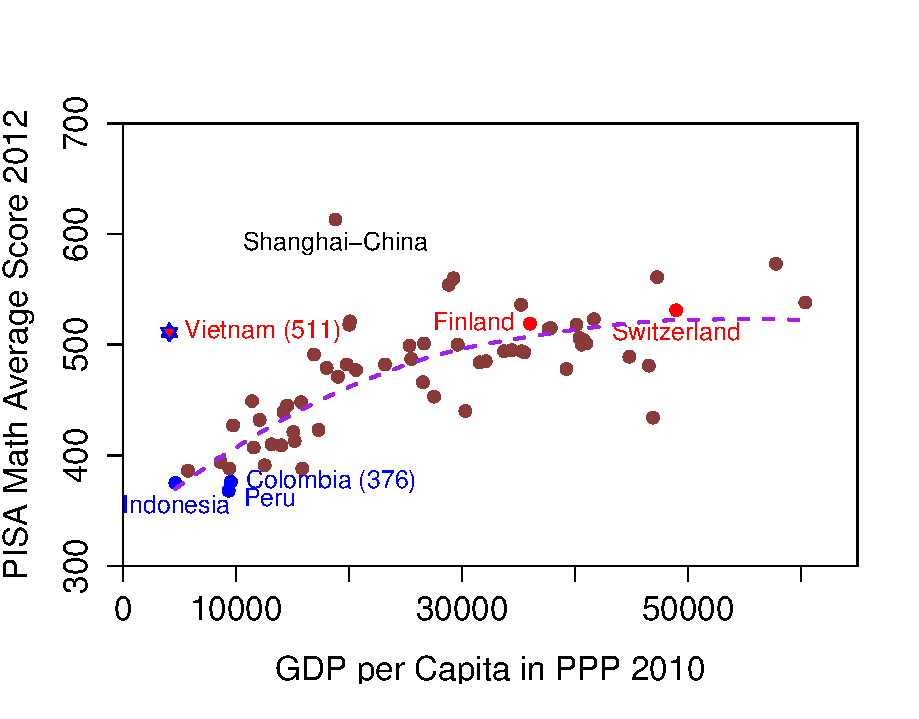
\includegraphics[width=0.75 \textwidth]{INTRFIG1.pdf} \\
\scriptsize{Source:OECD-PISA database        \hspace{3in}     }
   \label{Figure 1} 
\end{figure}

In the OECD-PISA database, there are seven countries other than Vietnam with a per capita GDP (in PPP dollars) below US\$ 10,000 - Albania, Colombia, Indonesia, Jordan, Peru, Thailand and Tunisia.  Their collective weighted average performance in mathematics was a mean score of 383. It is helpful to understand the significance of the 128 point difference with Vietnam. According to a recent OECD publication (\cite{OECD2013a}) \emph{"An entire proficiency level in mathematics spans about 70 score points \textendash  
a large difference in the skills and
knowledge students at that level possess. Such a gap represents the equivalent of about two years of schooling in the typical OECD country."}. Applying this heuristic would imply a nearly 3 year difference in attainment between Vietnam and the group of 7 developing countries in the PISA database. It should be noted at the outset that cross-section data from one instalment of PISA does not permit causal inference, but correlations can still provide useful insights. The difference is not only for mathematics and not just in the mean score, but spanning the entire test distribution, as can be seen in Figure 2. 

\begin{figure}[H]
\caption{Kernel Density comparison between Vietnam and other Developing Countries}\label{fig:Kernel}
         \centering
         \begin{subfigure}[b]{0.3\textwidth}
                 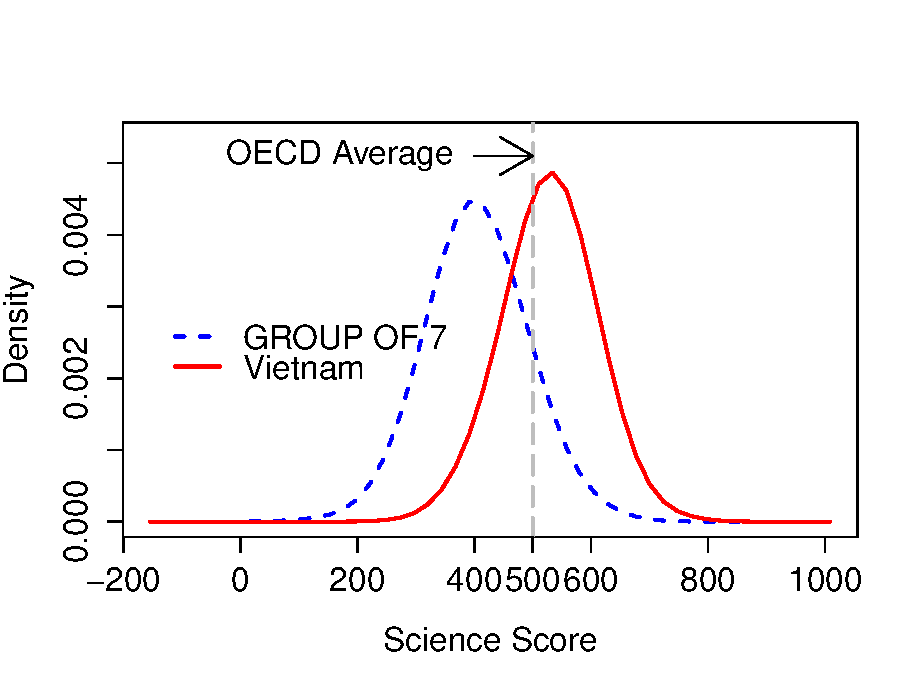
\includegraphics[width=\textwidth]{INTRFIG2a.pdf}
                 \caption{Science}
                 \label{fig:science}
         \end{subfigure}%
         ~ %add desired spacing between images, e. g. ~, \quad, \qquad, \hfill etc.
           %(or a blank line to force the subfigure onto a new line)
         \begin{subfigure}[b]{0.3\textwidth}
                 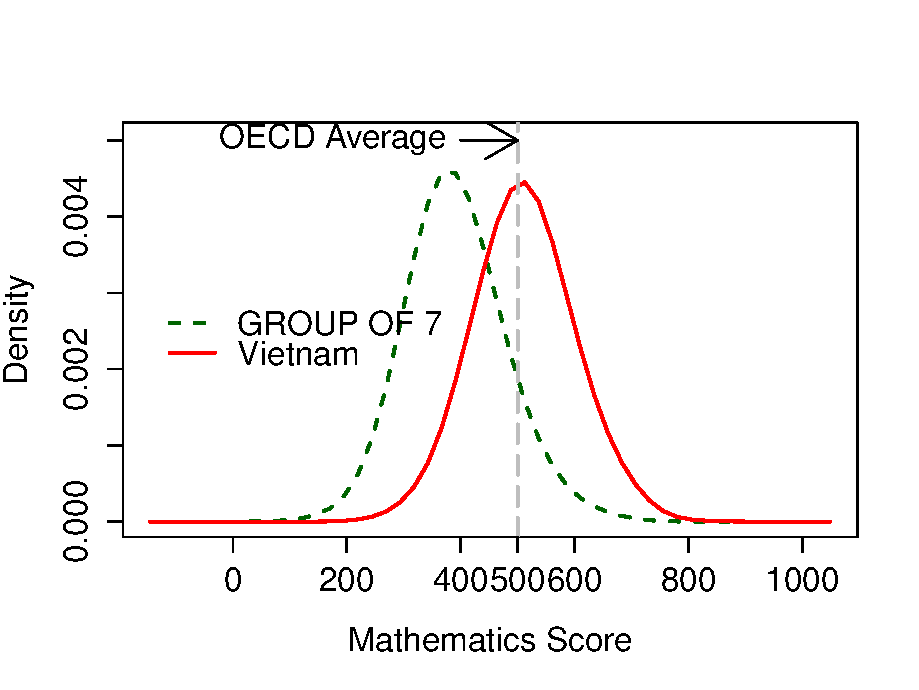
\includegraphics[width=\textwidth]{INTRFIG2b.pdf}
                 \caption{Mathematics}
                 \label{fig:mathematics}
         \end{subfigure}
         ~ %add desired spacing between images, e. g. ~, \quad, \qquad, \hfill etc.
           %(or a blank line to force the subfigure onto a new line)
         \begin{subfigure}[b]{0.28\textwidth}
                 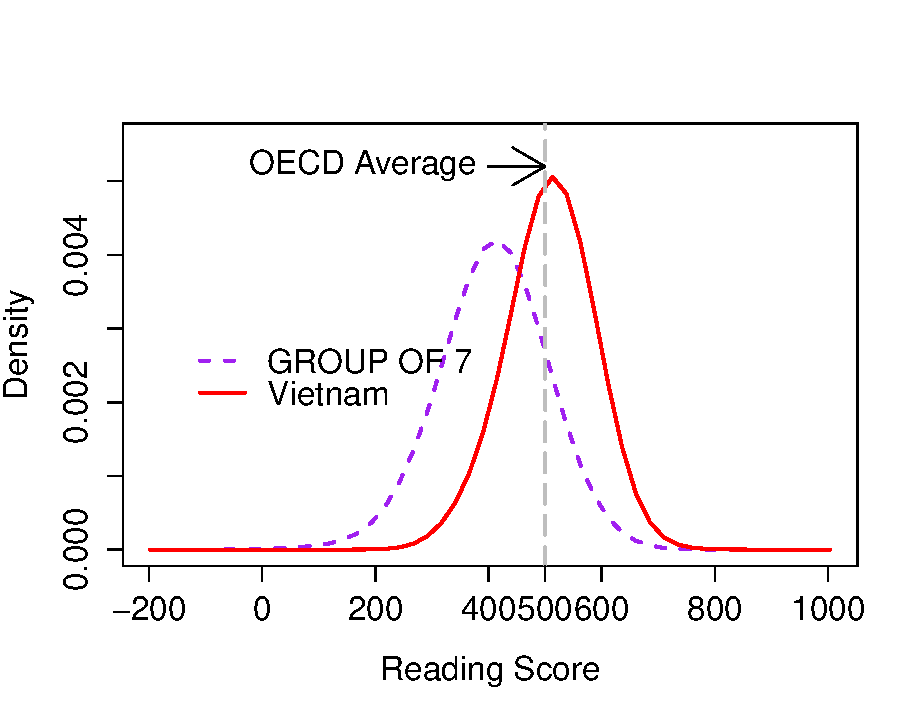
\includegraphics[width=\textwidth]{INTRFIG2c.pdf}
                 \caption{Reading}
                 \label{fig:reading}
         \end{subfigure}
     \end{figure}

A range of alternative classifications are possible to organize the possible explanatory factors available in the OECD-PISA database. Figure 3 presents four sets of factors, starting clockwise from the right.

\begin{figure}[H]
   \caption{Conceptual Scheme}
   \centering 
     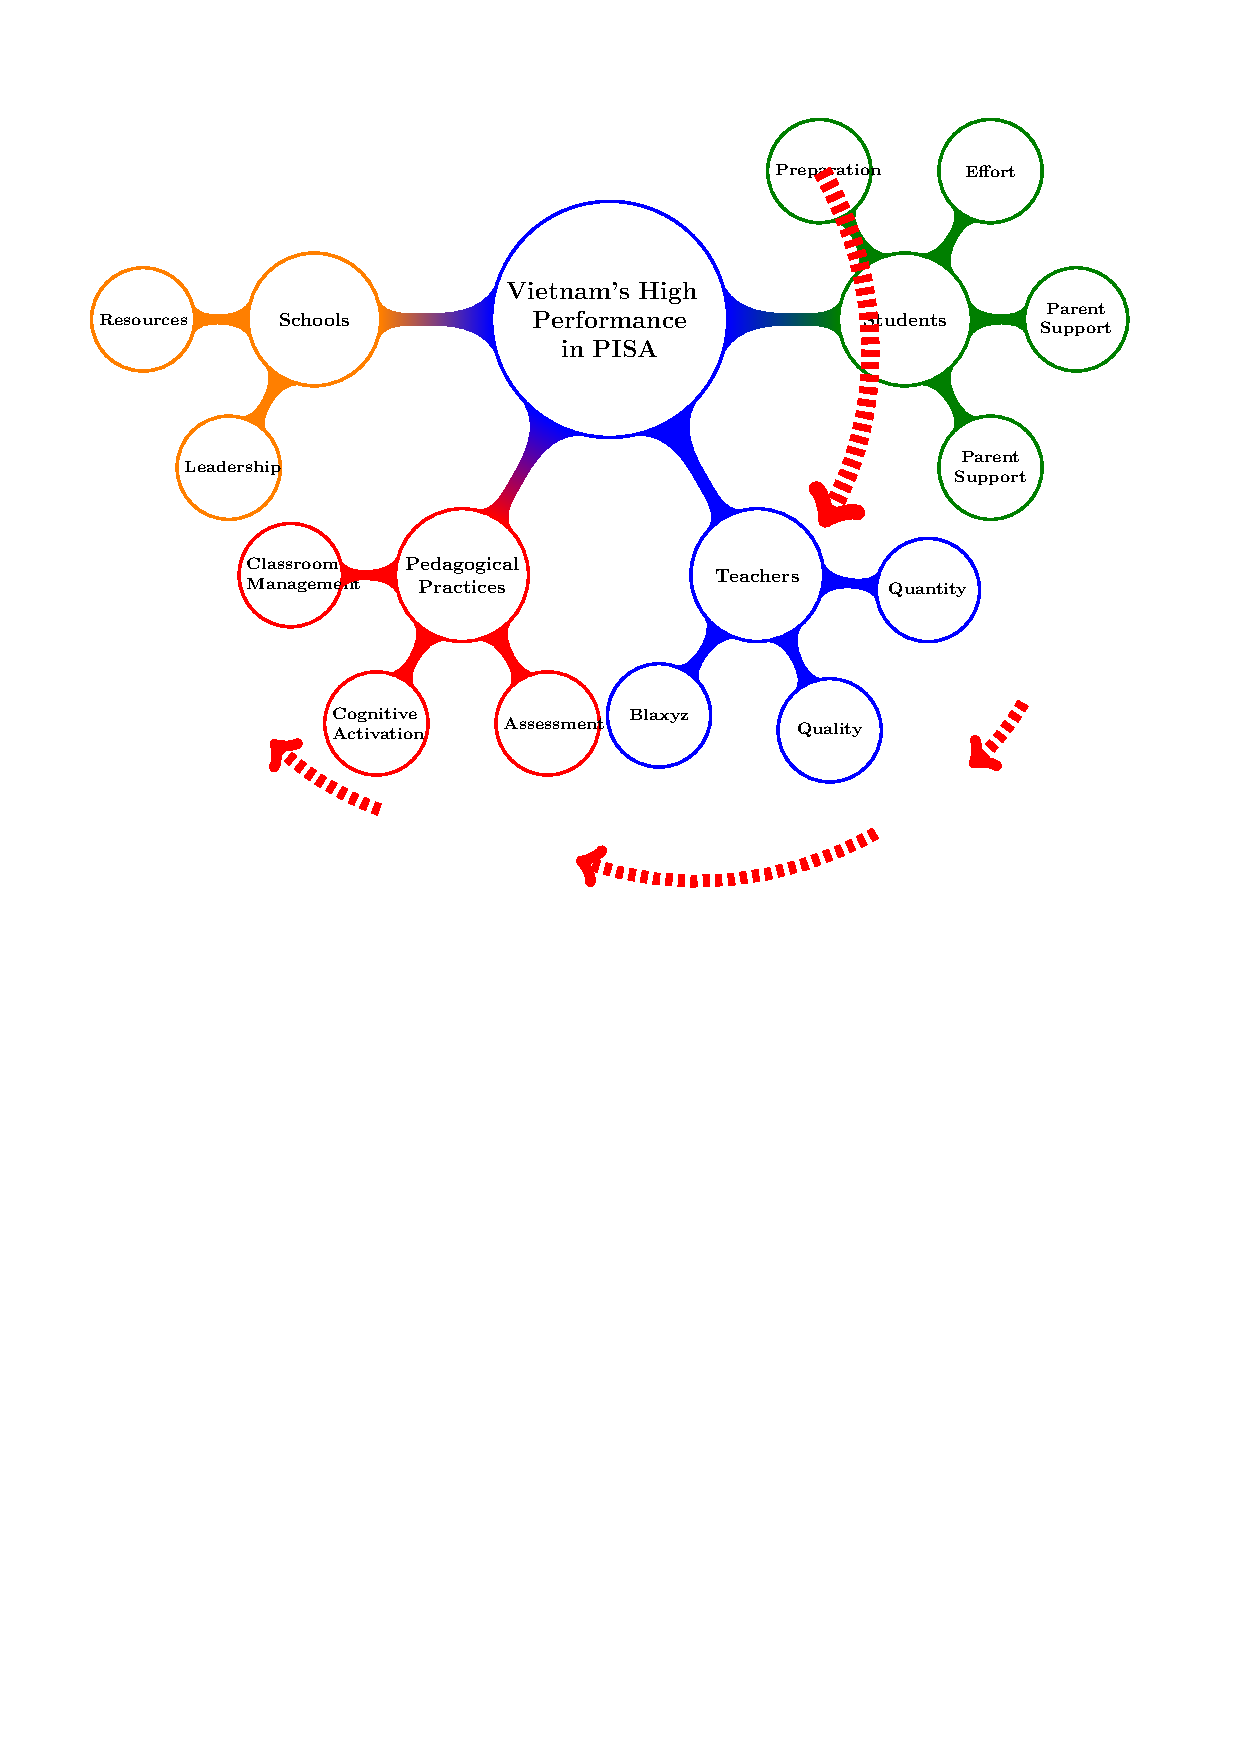
\includegraphics[width= 5in]{INTRTIKZ.pdf} \\
   \label{fig:m} 
\end{figure}

The structure of the paper is as follows. Student related variables, including the student's home environment are considered first in Section 2. Teachers related factors, together with teaching/pedagogical practices are discussed in Section 3. Section 4 considers the last factors, school type and resources and school leadership. These sections of this paper presents a descriptive and analytical comparison of these factors in a comparative context, comparing the 7 countries (henceforth, Dev7) with Vietnam. Section 5 presents some conclusions from the study, including directions for further research.
 
\section{What student related factors explain the achivevement gap of Vietnam ?}

The OECD-PISA initiative includes questionnaires administered to students and to school authorities. These questionnaires are fairly detailed and are described in the OECD-PISA documentation. In addition to the questionnaire items, the OECD-PISA team has also generated a range of indices from the underlying questions. These indices are sometime simple numerical compilations and sometimes the result of analysis such as principal-components analysis to combine different items. The constructed indices are carefully checked for validity and reliability against the whole database, including OECD and non-OECD countries. The availability of the constructed variables greatly facilitates the analysis of OECD-PISA data. An example is the case of the measure of the student's household material well-being termed as WEALTH, which is comprised from student's reported family ownership of durables and the condition of the student's dwelling. Bath room room?\\
It is possible that Vietnamese students, raised under a culture with high values for discipline and respect for authority, are better performers.Dalton and Ong, 2005(\cite{DaltonOng05}).

\subsection{Student Characteristics and Background}

\begin{table}[H]
	\tiny
	\def\arraystretch{0.9}
	\centering
	\caption{Summary statistics - student characteristics and background}
	\begin{tabulary}{1.0\textwidth}{L L C C C C}
		\hline\hline \\
		\multicolumn{2}{c}{}
		& \multicolumn{2}{c}{Dev7 countries}
		& \multicolumn{2}{c}{Vietnam}	\\
		\hline & & & & & & 
		Variable & Description & MS & Valid N &  MS & Valid N \\
		\hline \\
		FEMALE & Sex of student & 0.5265 & 41394 & 0.5336 & 4882 \\ 
		& & (0.4993) &  & (0.4989) &  \\ 
		PRESCHOOL & Attend Preschool & 0.7888 & 40114 & 0.912 & 4866 \\ 
		& (ISCED 0) & (0.4082) &  & (0.2833) &  \\ 
		REPEAT & Grade repeating & 0.1915 & 40343 & 0.0679 & 4860 \\ 
		& &  (0.3935) &  & (0.2516) &  \\ 
		ST08Q01 & Times late & 1.5131 & 40663 & 1.1872 & 4873 \\ 
		& for school & (0.7648) &  & (0.4685) &  \\ 
		ST09Q01 & Days unexcused & 1.2192 & 40650 & 1.0999 & 4875 \\ 
		& absence & (0.5276) &  & (0.3527) &  \\ 
		ST115Q01 & Times skipped & 1.2585 & 40632 & 1.0764 & 4880 \\ 
		& classes & (0.545) &  & (0.3216) &  \\ 
		HISEI & Highest parental & 40.4196 & 32814  & 26.6023 & 4860 \\ 
		& occupational status & (22.5168) &  & (19.855) &  \\ 
		MISCED & Educational level & 3.1193 & 40486 & 2.1744 & 4844 \\ 
		& of mother (ISCED) & (1.9853) &  & (1.6059) &  \\ 
		WEALTH & Family wealth & -1.4606 & 40821 & -2.1343 & 4881 \\ 
		& possessions & (1.2267) &  & (1.1656) &  \\ 
		CULTPOS & Cultural possessions & -0.1424 & 39905 & -0.2361 & 4809 \\ 
		& & (0.9678) &  & (1.0173) &  \\ 
		HEDRES & Home educational &  -0.7427 & 40579 & -1.0743 & 4874 \\ 
		& resources & (1.1473) &  & (0.9364) &  \\ 
		BOOK\_N & Number of books & 53.6393 & 39631 & 50.786 & 4841 \\ 
		& in family home & (94.5556) &  & (75.4031) &  \\
		\hline \\
	\multicolumn{6}{l}{Notes: The variables relate to the questionnaires administered to students in the general}\\    
	\multicolumn{6}{l}{(non-rotated) booklet. For a more detailed description of variables, please see Table xx.}\\
	\multicolumn{6}{l}{Items marked with \textit{(r)} are taken from the rotated student questionnaire. The variable}\\
	\multicolumn{6}{l}{means of Dev7 and Vietnam are statistically different at the 5\% significance level, except}\\
	\multicolumn{6}{l}{FEMALE.}\\
\end{tabulary}
\end{table}

Lorem ipsum dolor sit amet, consectetur adipiscing elit. Pellentesque ut lacus nec sapien volutpat tempus vitae et lorem.

\subsection{Student Effort}

\begin{table}[H]
	\tiny
	\def\arraystretch{0.9}
	\centering
	\caption{Summary statistics - student effort}
	\begin{tabulary}{1.0\textwidth}{L L C C C C}
		\hline\hline \\
		\multicolumn{2}{c}{}
		& \multicolumn{2}{c}{Dev7 countries}
		& \multicolumn{2}{c}{Vietnam}	\\
		\hline & & & & & & 
		Variable & Description & MS & Valid N &  MS & Valid N \\
		\hline \\
		MATWKETH \textit{(r)} & Mathematics & 0.4514 & 26140 & -0.0014 & 3217 \\ 
		& work ethic & (0.9782) &  & (0.6915) &  \\ 
		OUTMATH\_NONE \textit{(r)} & Weekly out-of-school &  0.4024 & 23603 & 0.1745 & 3227 \\ 
		& lessons in math & (0.4904) &  & (0.3796) &  \\ 
		OUTMATH\_LESS2 \textit{(r)} & Weekly out-of-school & 0.222 & 23603 & 0.1701 & 3227 \\ 
		& lessons in math  & (0.4156) &  & (0.3758) &  \\ 
		OUTMATH\_2TO4 \textit{(r)} & Weekly out-of-school & 0.2041 & 23603 & 0.2993 & 3227 \\ 
		& lessons in math  & (0.4031) &  & (0.458) &  \\ 
		OUTMATH\_4TO6 \textit{(r)} & Weekly out-of-school & 0.1034 & 23603 & 0.2151 & 3227 \\ 
		& lessons in math  & (0.3045) &  & (0.4109) &  \\ 
		OUTREAD\_NONE \textit{(r)} & Weekly out-of-school & 0.554 & 23531 & 0.4732 & 3223 \\ 
		& lessons in reading  & (0.4971) &  & (0.4994) &  \\ 
		OUTREAD\_LESS2 \textit{(r)} & Weekly out-of-school & 0.1886 & 23531 & 0.2119 & 3223 \\ 
		& lessons in reading  & (0.3912) &  & (0.4087) &  \\ 
		OUTREAD\_2TO4 \textit{(r)} & Weekly out-of-school & 0.1419 & 23531 & 0.2023 & 3223 \\ 
		& lessons in reading  & (0.349) &  & (0.4018) &  \\ 
		OUTREAD\_4TO6 \textit{(r)} & Weekly out-of-school & 0.0673 & 23531 & 0.0794 & 3223 \\ 
		& lessons in reading  & (0.2506) &  & (0.2704) &  \\ 
		OUTSCIE\_NONE \textit{(r)} & Weekly out-of-school & 0.4679 & 23298 & 0.327 & 3205 \\ 
		& lessons in science  & (0.499) &  & (0.4692) &  \\ 
		OUTSCIE\_LESS2 \textit{(r)} & Weekly out-of-school &  0.211 & 23298 & 0.2387 & 3205 \\ 
		& lessons in science  & (0.408) &  & (0.4263) &  \\ 
		OUTSCIE\_2TO4 \textit{(r)} & Weekly out-of-school & 0.181 & 23298 & 0.2293 & 3205 \\ 
		& lessons in science  & (0.385) &  & (0.4205) &  \\ 
		OUTSCIE\_4TO6 \textit{(r)} & Weekly out-of-school & 0.0867 & 23298 & 0.1345 & 3205 \\ 
		& lessons in science  & (0.2815) &  & (0.3412) &  \\
		ST57Q01 \textit{(r)} & Out-of-school time & 5.0953 & 23696 & 5.8145 & 3164 \\ 
		& homework & (5.0319) &  & (5.7196) &  \\ 
		ST57Q02 \textit{(r)} & Out-of-school time & 2.551 & 19355 & 2.8814 & 2285 \\ 
		& guided homework & (2.9296) &  & (3.2384) &  \\ 
		ST57Q03 \textit{(r)} & Out-of-school time & 1.7276 & 20367 & 1.5749 & 3049 \\ 
		& personal tutor & (2.7884) &  & (2.938) &  \\
		ST57Q04 \textit{(r)} & Out-of-school time & 1.892 & 19517 & 4.878 & 3091 \\ 
		& classes by company & (3.3487) &  & (4.8058) &  \\ 
		ST57Q05 \textit{(r)} & Out-of-school time & 2.1354 & 21542 & 1.7646 & 3092 \\ 
		& parent/family member & (3.055) &  & (3.2442) &  \\ 
		ST57Q06 \textit{(r)} & Out-of-school time & 2.588 & 21338 & 1.8029 & 3079 \\ 
		& learn on computer & (3.5519) &  & (3.0496) &  \\ 
		\hline \\
		\multicolumn{6}{l}{Notes: The variables relate to the questionnaires administered to students in the rotated booklet.}\\   
		\multicolumn{6}{l}{For a more detailed description of variables, please see Table xx. Items marked with \textit{(r)} are}\\    
		\multicolumn{6}{l}{taken from the rotated student questionnaire. The variable means of Dev7 and Vietnam are}\\
		\multicolumn{6}{l}{statistically different at the 5\% significance level.}\\		
	\end{tabulary}
\end{table}

Vivamus elementum, dolor suscipit elementum rutrum, lorem tellus fermentum diam, venenatis ultricies orci urna a ex. Duis aliquam placerat velit, luctus venenatis mi hendrerit vel. In eu risus et ligula molestie iaculis.

\subsection{Student Attitude}

\begin{table}[H]
	\tiny
	\def\arraystretch{0.9}
	\centering
	\caption{Summary statistics - student attitude}
	\begin{tabulary}{1.0\textwidth}{L L C C C C}
		\hline\hline \\
		\multicolumn{2}{c}{}
		& \multicolumn{2}{c}{Dev7 countries}
		& \multicolumn{2}{c}{Vietnam}	\\
		\hline & & & & & & 
		Variable & Description & MS & Valid N &  MS & Valid N \\
		\hline \\
		INSTMOT \textit{(r)} & Instrumental & 0.4253 & 26566 & 0.3683 & 3220 \\ 
		& motivation for math & (0.8558) &  & (0.7289) &  \\ 
		INTMAT \textit{(r)} & Interest in & 0.7212 & 26634 & 0.6927 & 3219 \\ 
		& mathematics & (0.8533) &  & (0.6636) &  \\ 
		SUBNORM \textit{(r)} & Subjective norms & 0.716 & 26509 & -0.0923 & 3220 \\ 
		& in mathematics & (1.165) &  & (0.8395) &  \\ 
		MATHEFF \textit{(r)} & Self-Efficacy & -0.2269 & 26457 & -0.2655 & 3217 \\ 
		& in mathemtatics & (0.8516) &  & (0.6363) &  \\ 		
		FAILMAT \textit{(r)} & Attributions to & 0.083 & 26155 & 0.0895 & 3214 \\ 
		& failure in math & (1.0312) &  & (0.6319) &  \\ 
		MATINTFC \textit{(r)} & Mathematics & 0.092 & 24827 & 0.3285 & 3181 \\ 
		& intentions & (0.9837) &  & (1.0964) &  \\ 
		MATBEH \textit{(r)} & Mathematics & 0.8764 & 25899 & 0.6757 & 3211 \\ 
		& behaviour & (0.9697) &  & (0.6408) &  \\ 
		PERSEV \textit{(r)} & Perseverance & 0.3387 & 25710 & 0.4475 & 3211 \\ 
		& in problem solving & (0.9605) &  & (0.8767) &  \\ 
		OPENPS \textit{(r)} & Openness to & 0.1949 & 25612 & -0.6125 & 3207 \\ 
		& problem solving & (0.9787) &  & (0.8708) &  \\ 
		SCMAT \textit{(r)} & Self-concept of & 0.1673 & 26222 & -0.1896 & 3249 \\ 
		&  own math skills & (0.8101) &  & (0.5903) &  \\ 
		ANXMAT \textit{(r)} & Mathematics & 0.3995 & 26275 & 0.2115 & 3248 \\ 
		& Anxiety & (0.7724) &  & (0.6354) &  \\ 
		BELONG \textit{(r)} & Sense of & 0.0511 & 25785 & -0.2574 & 3253 \\ 
		& belonging to school & (0.9428) &  & (0.7032) &  \\ 
		ATSCHL \textit{(r)} & Attitude - school & 0.1616 & 25563 & 0.143 & 3246 \\ 
		& learning is useful  & (0.9986) &  & (0.8648) &  \\ 
		ATTLNACT \textit{(r)} & Attitude - Trying hard & 0.1233 & 25368 & -0.535 & 3248 \\ 
		& at school pays off & (0.964) &  & (0.8212) &  \\ 
		ATT\_CONTROL \textit{(r)} & Perceived control & 0.8507 & 25106 & 0.6608 & 3228 \\ 
		& over grades & (0.3564) &  & (0.4735) &  \\ 	
		\hline \\
		\multicolumn{6}{l}{Notes: The variables relate to the questionnaires administered to students in the rotated booklet.}\\   
		\multicolumn{6}{l}{For a more detailed description of variables, please see Table xx. Items marked with \textit{(r)} are}\\    
		\multicolumn{6}{l}{taken from the rotated student questionnaire. The variable means of Dev7 and Vietnam are}\\
		\multicolumn{6}{l}{statistically different at the 5\% significance level, except FAILMAT and ATTSCHL.}\\	
\end{tabulary}
\end{table}

Quisque pulvinar at lorem vel lobortis. Duis tempor, sem in dignissim facilisis, libero nisi convallis mi, ac dictum lectus eros nec lacus.

\subsection{Student Experience in Mathematics}
These are all student self-reported items, asked in rotational part 2. 

\begin{table}[H]
	\tiny
	\def\arraystretch{0.9}
	\centering
	\caption{Summary statistics - student experience in mathematics}
	\begin{tabulary}{1.0\textwidth}{L L C C C C}
		\hline\hline \\
		\multicolumn{2}{c}{}
		& \multicolumn{2}{c}{Dev7 countries}
		& \multicolumn{2}{c}{Vietnam}	\\
		\hline & & & & & & 
		Variable & Description & MS & Valid N &  MS & Valid N \\
		\hline \\		
		EXAPPLM \textit{(r)} & Experience with & 0.1111 & 26133 & -0.2418 & 3243 \\ 
		& applied math tasks & (1.06) &  & (0.7624) &  \\ 
		EXPUREM \textit{(r)} & Experience with pure & -0.1384 & 25973 & 0.1587 & 3244 \\ 
		& math tasks & (0.9809) &  & (0.8076) &  \\ 
		FAMCONC \textit{(r)} & Familiarity with & -0.5441 & 25832 & 0.4297 & 3231 \\ 
		& math concepts & (0.8768) &  & (0.9057) &  \\ 	
		\hline \\
		\multicolumn{6}{l}{Notes: The variables relate to the questionnaires administered to students in the rotated}\\   
		\multicolumn{6}{l}{booklet. For a more detailed description of variables, please see Table xx. Items marked}\\    
		\multicolumn{6}{l}{with \textit{(r)} are taken from the rotated student questionnaire. The variable means of}\\
		\multicolumn{6}{l}{Dev7 and Vietnam are statistically different at the 5\% significance level.}\\
\end{tabulary}
\end{table}

\subsection{Home Support} 

\begin{table}[H]
	\tiny
	\def\arraystretch{0.9}
	\centering
	\caption{Summary statistics - student experience in mathematics}
	\begin{tabulary}{1.0\textwidth}{L L C C C C}
		\hline\hline \\
		\multicolumn{2}{c}{}
		& \multicolumn{2}{c}{Dev7 countries}
		& \multicolumn{2}{c}{Vietnam}	\\
		\hline & & & & & & 
		Variable & Description & MS & Valid N &  MS & Valid N \\
		\hline \\
		PARPRESSURE & Parental achievement & 0.2665 & 40372 & 0.3837 & 4866 \\ 
		& pressure & (0.4421) &  & (0.4863) &  \\  
		TIGERMOM & Parent initiates - &  52.4472 & 41394 & 62.4183 & 4882 \\ 
		& progress discussion & (38.097) &  & (41.3743) &  \\ 
		VOLUMOM & Parent Participation - & 35.2134 & 41394 & 38.3623 & 4882 \\ 
		& Volunteering & (38.8428) &  & (39.9773) &  \\ 
		TEACHMOM & Parent Participation - & 12.1764 & 41394 & 38.2821 & 4882 \\ 
		& Teaching Assistance & (23.4241) &  & (41.5357) &  \\ 
		FUNDMOM & Parent Participation - & 23.0784 & 41394 & 59.6022 & 4882 \\ 
		& Fundraising & (35.2134) &  & (44.0376) &  \\ 
		COUNCILMOM & Parent Participation - & 36.4546 & 41394 & 23.1174 & 4882 \\ 
		& School government & (37.2252) &  & (36.4406) &  \\
		BKGR\_FAMPROB \textit{(r)} & Home problems - & 0.4705 & 25038 & 0.264 & 3231 \\ 
		& deter effort in school & (0.4991) &  & (0.4409) &  \\
		\hline \\
		\multicolumn{6}{l}{Notes: The variables relate to the questionnaires administered to students in the rotated booklet}\\   
		\multicolumn{6}{l}{and the general (non-rotated) booklet. For a more detailed description of variables, please see}\\    
		\multicolumn{6}{l}{Table xx. Items marked with \textit{(r)} are taken from the rotated student questionnaire. The variable}\\
		\multicolumn{6}{l}{means of Dev7 and Vietnam are statistically different at the 5\% significance level.}\\	
	\end{tabulary}
	\end{table}

Nunc feugiat nisi sit amet elit condimentum iaculis. Nunc porttitor purus non semper tristique. Curabitur ac convallis nunc, at maximus orci.

\section{What teacher and teaching/pedagogical practices related factors explains the achivevement gap of Vietnam ?}

\subsection{Teachers - Characteristics and Quantitative Measures} 

\begin{table}[H]
	\tiny
	\def\arraystretch{0.9}
	\centering
	\caption{Summary statistics - teacher characteristics and quantitative measures}
	\begin{tabulary}{1.0\textwidth}{L L C C C C}
		\hline\hline \\
		\multicolumn{2}{c}{}
		& \multicolumn{2}{c}{Dev7 countries}
		& \multicolumn{2}{c}{Vietnam}	\\
		\hline & & & & & & 
		Variable & Description & MS & Valid N &  MS & Valid N \\
		\hline \\
		STRATIO & Student-teacher ratio & 19.715 & 33742 & 18.9656 & 4743 \\ 
		& & (9.4135) &  & (5.5255) &  \\ 
		PROPCERT & Proportion of & 0.6757 & 35130 & 0.7961 & 4586 \\ 
		& certified teacher & (0.4042) &  & (0.3978) &  \\ 
		PROPQUAL & Proportion of teachers & 0.8756 & 36319 & 0.8775 & 4708 \\ 
		& with ISCED 5A & (0.2181) &  & (0.2758) &  \\ 
		SMRATIO & Mathematics & 188.1791 & 33985 & 120.9773 & 4777 \\ 
		& teacher-student ratio & (158.6256) &  & (43.6092) &  \\ 
		TCSHORT & Shortage of & 0.4846 & 41077 & 0.4249 & 4882 \\ 
		& teaching staff & (1.2627) &  & (1.1636) &  \\ 
		LHRS \textit{(r)} & Taught hours of & 3.599 & 22177 & 3.2207 & 2870 \\ 
		& 'test language' &(1.9887) &  & (1.1576) &  \\ 
		SHRS \textit{(r)} & Taught hours of & 3.7566 & 21701 & 3.9597 & 2473 \\ 
		& science & (2.5078) &  & (2.5484) &  \\ 
		MHRS \textit{(r)} & Taught hours of & 3.896 & 21913 & 3.7878 & 2850 \\ 
		& mathematics & (2.0335) &  & (1.3764) &  \\ 
		\hline \\
		\multicolumn{6}{l}{Notes: The variables relate to the questionnaires administered to principals (schools) and}\\    
		\multicolumn{6}{l}{students in the rotated booklet. For a more detailed description of variables, please see}\\
		\multicolumn{6}{l}{Table xx. Items marked with \textit{(r)} are taken from the rotated student questionnaire. The}\\
		\multicolumn{6}{l}{variable means of Dev7 and Vietnam are statistically different at the 5\% significance level,}\\
		\multicolumn{6}{l}{except PROPQUAL.}\\
	\end{tabulary}
	\end{table}

Maecenas ullamcorper massa nec faucibus cursus. Aenean porttitor augue nec rhoncus bibendum. Cras venenatis, ex et commodo consequat, sem arcu suscipit lacus, id efficitur odio purus non felis.

\subsection{Teachers - Quality} 

\begin{table}[H]
	\tiny
	\def\arraystretch{0.9}
	\centering
	\caption{Summary statistics - teacher quality}
	\begin{tabulary}{1.0\textwidth}{L L C C C C}
		\hline\hline \\
		\multicolumn{2}{c}{}
		& \multicolumn{2}{c}{Dev7 countries}
		& \multicolumn{2}{c}{Vietnam}	\\
		\hline & & & & & & 
		Variable & Description & MS & Valid N &  MS & Valid N \\
		\hline \\
		TCFOCST & Teacher focus & 0.4975 & 41370 & 0.1402 & 4882 \\ 
		& & (1.0056) &  & (0.8377) &  \\ 
		SC35Q02 & Professional development & 40.5068 & 39550 & 49.0086 & 4762 \\ 
		& in math in last 3 months & (40.8546) &  & (45.1706) &  \\ 
		TCH\_MENT & Teacher mentoring & 0.8566 & 40734 & 0.9859 & 4882 \\ 
		& as quality assurance & (0.3505) &  & (0.1181) &  \\ 
		MTSUP \textit{(r)} & Mathematics supportive & 0.4778 & 25918 & 0.3685 & 3247 \\ 
		& teaching style & (0.9613) &  & (0.774) &  \\ 
		STUDREL \textit{(r)} & Teacher student & 0.3794 & 25870 & 0.0186 & 3253 \\ 
		& relations & (1.0178) &  & (0.8883) &  \\ 
		TCHQUAL\_DIFF \textit{(r)} & with different teacher & 0.5249 & 24986 & 0.363 & 3231 \\ 
		& student would work harder & (0.4994) &  & (0.481) &  \\  
		TCH\_INCENTV & teacher appraisal led &  -0.0317 & 41394 & 0.2687 & 4882 \\ 
		& to gratification & (1.0301) &  & (0.6336) &  \\ 	
		\multicolumn{6}{l}{\textit{Quality assurance of mathematics teachers through ...}} \\[0.5em]
		TCM\_STUASS & test or assessment &  0.8762 & 41110 & 0.9818 & 4882 \\ 
		& of student achievement & (0.3293) &  & (0.1338) &  \\ 
		TCM\_PEER & teacher peer review & 0.7916 & 41095 & 0.8382 & 4882 \\ 
		& of lectures, methods etc & (0.4061) &  & (0.3683) &  \\ 
		TCM\_OBSER & principal or senior & 0.8015 & 41170 & 0.9785 & 4882 \\ 
		& staff observations & (0.3989) &  & (0.1451) &  \\ 
		TCM\_INSPE & obersavtion of classes & 0.5882 & 41020 & 0.8664 & 4882 \\ 
		& external inspector & (0.4922) &  & (0.3402) &  \\ 
		\hline \\
		\multicolumn{6}{l}{Notes: The variables relate to the questionnaires administered to principals (schools) and}\\    
		\multicolumn{6}{l}{students in the rotated booklet. For a more detailed description of variables, please see}\\
		\multicolumn{6}{l}{Table xx. Items marked with \textit{(r)} are taken from the rotated student questionnaire. The}\\
		\multicolumn{6}{l}{variable means of Dev7 and Vietnam are statistically different at the 5\% significance level,}\\
		\multicolumn{6}{l}{except PROPQUAL.}\\	
	\end{tabulary}
	\end{table}

Praesent malesuada et mi id cursus. Nam elit enim, molestie ac nulla vel, bibendum sollicitudin ex. Suspendisse sit amet erat vitae mauris fermentum tincidunt in at nulla.

\subsection{Pedagogical/Teaching practices in Mathematics} 

\begin{table}[H]
	\tiny
	\def\arraystretch{0.9}
	\centering
	\caption{Summary statistics - pedagogical/teaching practices in Mathematics}
	\begin{tabulary}{1.0\textwidth}{L L C C C C}
		\hline\hline \\
		\multicolumn{2}{c}{}
		& \multicolumn{2}{c}{Dev7 countries}
		& \multicolumn{2}{c}{Vietnam}	\\
		\hline & & & & & & 
		Variable & Description & MS & Valid N &  MS & Valid N \\
		\hline \\
		COMP\_USE & Math policy - use of & 0.4345 & 40800 & 0.6447 & 4815 \\ 
		& computers in class & (0.4957) &  & (0.4787) &  \\ 
		TXT\_BOOK & Math policy - & 0.7905 & 40557 & 0.7855 & 4882 \\ 
		& same textbook & (0.4069) &  & (0.4105) &  \\ 
		STD\_CUR & Maths policy - & 0.8705 & 40595 & 0.949 & 4882 \\ 
		& standardized curriculum & (0.3358) &  & (0.22) &  \\ 
		TCHBEHTD \textit{(r)}& Teacher oriented & 0.4973 & 26433 & 0.2964 & 3254 \\ 
		& inctruction method & (1.0798) &  & (0.8099) &  \\ 
		TCHBEHSO \textit{(r)} & Student oriented & 0.7921 & 26358 & 0.2969 & 3248 \\ 
		& instruction method & (0.9545) &  & (0.819) &  \\ 
		\hline \\
		\multicolumn{6}{l}{Notes: The variables relate to the questionnaires administered to principals (schools) and}\\    
		\multicolumn{6}{l}{students in the rotated booklet. For a more detailed description of variables, please see}\\
		\multicolumn{6}{l}{Table xx. Items marked with \textit{(r)} are taken from the rotated student questionnaire. The}\\
		\multicolumn{6}{l}{variable means of Dev7 and Vietnam are statistically different at the 5\% significance level,}\\
		\multicolumn{6}{l}{except TXT\_BOOK.}\\
	\end{tabulary}
	\end{table}

Suspendisse non justo et diam bibendum pulvinar. Sed id tortor posuere, rhoncus justo at, facilisis arcu. Duis eleifend fermentum tortor, eget laoreet sem varius ac.

\subsection{Formative Assessment of Students} 

\begin{table}[H]
	\tiny
	\def\arraystretch{0.9}
	\centering
	\caption{Summary statistics - formative assessment of students}
	\begin{tabulary}{1.0\textwidth}{L L C C C C}
		\hline\hline \\
		\multicolumn{2}{c}{}
		& \multicolumn{2}{c}{Dev7 countries}
		& \multicolumn{2}{c}{Vietnam}	\\
		\hline & & & & & & 
		Variable & Description & MS & Valid N &  MS & Valid N \\
		\hline \\
		\multicolumn{6}{l}{\textit{Assessment used to}} \\[0.5em]
		ASS\_PROG & inform parents & 0.9695 & 40708 & 0.9928 & 4882 \\ 
		& about childs progress & (0.172) &  & (0.0844) &  \\ 
		ASS\_PROM & decide on students’ & 0.8988 & 40483 & 0.9508 & 4882 \\ 
		& retention or promotion & (0.3016) &  & (0.2162) &  \\ 
		ASS\_INSTR & group students for & 0.6648 & 40316 & 0.7378 & 4882 \\ 
		&  instructional purposes & (0.4721) &  & (0.4399) &  \\ 
		ASS\_NAT & compare school to & 0.7008 & 40493 & 0.8785 & 4882 \\ 
		& national performance & (0.4579) &  & (0.3267) &  \\ 
		ASS\_SCH & monitor the schools & 0.9111 & 40555 & 0.9799 & 4882 \\ 
		& yearly progress & (0.2846) &  & (0.1403) &  \\ 
		ASS\_TCH & make judgements on & 0.7764 & 40400 & 0.9912 & 4882 \\ 
		& teachers' effectiveness & (0.4166) &  & (0.0934) &  \\ 
		ASS\_CUR & identify improvements & 0.9017 & 40586 & 0.9127 & 4882 \\ 
		& in the curriculum & (0.2977) &  & (0.2822) &  \\ 
		ASS\_OTH & compare school with & 0.661 & 40386 & 0.866 & 4882 \\ 
		& other schools & (0.4734) &  & (0.3406) &  \\ 
		TCHBEHFA \textit{(r)} & help students perform &  0.4634 & 26245 & 0.005 & 3246 \\ 
		& better & (0.9934) &  & (0.79) &  \\ 
		\hline \\
		\multicolumn{6}{l}{Notes: The variables relate to the questionnaires administered to principals (schools) and}\\    
		\multicolumn{6}{l}{students in the rotated booklet. For a more detailed description of variables, please see}\\
		\multicolumn{6}{l}{Table xx. Items marked with \textit{(r)} are taken from the rotated student questionnaire. The}\\
		\multicolumn{6}{l}{variable means of Dev7 and Vietnam are statistically different at the 5\% significance level.}\\	
	\end{tabulary}
	\end{table}

Quisque quis sapien commodo, molestie dolor nec, tincidunt quam. Praesent at interdum nibh. Phasellus congue vehicula pulvinar. Aenean vel mattis velit.

\subsection{Cognitive Activation} 

\begin{table}[H]
	\tiny
	\def\arraystretch{0.9}
	\centering
	\caption{Summary statistics - cognitive activation}
	\begin{tabulary}{1.0\textwidth}{L L C C C C}
		\hline\hline \\
		\multicolumn{2}{c}{}
		& \multicolumn{2}{c}{Dev7 countries}
		& \multicolumn{2}{c}{Vietnam}	\\
		\hline & & & & & & 
		Variable & Description & MS & Valid N &  MS & Valid N \\
		\hline \\
		COGACT \textit{(r)} & Cognitive activation in & 0.2998 & 26217 & -0.3278 & 3249 \\ 
		& mathematics lessons & (0.975) &  & (0.6647) &  \\ 
		\hline \\
		\multicolumn{6}{l}{Notes: The variables relate to the questionnaires administered to principals (schools) and}\\    
		\multicolumn{6}{l}{students in the rotated booklet. For a more detailed description of variables, please see}\\
		\multicolumn{6}{l}{Table xx. Items marked with \textit{(r)} are taken from the rotated student questionnaire. The}\\
		\multicolumn{6}{l}{variable means of Dev7 and Vietnam are statistically different at the 5\% significance level.}\\
	\end{tabulary}
	\end{table}

Duis eu risus leo. Duis maximus ultrices eleifend. Quisque arcu sem, cursus nec condimentum nec, maximus ut nunc. Duis tempor massa ut enim tincidunt ullamcorper. 

\subsection{Classroom Management}

\begin{table}[H]
	\tiny
	\def\arraystretch{0.9}
	\centering
	\caption{Summary statistics - cognitive activation}
	\begin{tabulary}{1.0\textwidth}{L L C C C C}
		\hline\hline \\
		\multicolumn{2}{c}{}
		& \multicolumn{2}{c}{Dev7 countries}
		& \multicolumn{2}{c}{Vietnam}	\\
		\hline & & & & & & 
		Variable & Description & MS & Valid N &  MS & Valid N \\
		\hline \\
		STU\_FEEDB & Seeking written feed- &  0.7105 & 40788 & 0.8419 & 4882 \\ 
		& back from students & (0.4536) &  & (0.3649) &  \\ 
		CLSMAN \textit{(r)} & Teacher classroom & 0.2394 & 25753 & 0.2163 & 3252 \\ 
		& management & (0.905) &  & (0.7761) &  \\ 
		DISCLIMA \textit{(r)} & Disciplinary climate &  -0.0243 & 26242 & 0.3747 & 3254 \\ 
		& in class & (0.9055) &  & (0.6926) &  \\
		\hline \\
		\multicolumn{6}{l}{Notes: The variables relate to the questionnaires administered to principals (schools) and}\\    
		\multicolumn{6}{l}{students in the rotated booklet. For a more detailed description of variables, please see}\\
		\multicolumn{6}{l}{Table xx. Items marked with \textit{(r)} are taken from the rotated student questionnaire. The}\\
		\multicolumn{6}{l}{variable means of Dev7 and Vietnam are statistically different at the 5\% significance level,}\\
		\multicolumn{6}{l}{except CLSMAN.}\\
	\end{tabulary}
	\end{table}

Etiam a molestie mi, vitae porttitor metus. Donec in feugiat purus. Nam metus sem, placerat nec placerat et, posuere at turpis. Maecenas nec finibus nisl, nec rutrum elit. 

\section{What school related factors explains the achivevement gap of Vietnam ?}

\subsection{School Characteristics} 

\begin{table}[H]
	\tiny
	\def\arraystretch{0.9}
	\centering
	\caption{Summary statistics - school characteristics}
	\begin{tabulary}{1.0\textwidth}{L L C C C C}
		\hline\hline \\
		\multicolumn{2}{c}{}
		& \multicolumn{2}{c}{Dev7 countries}
		& \multicolumn{2}{c}{Vietnam}	\\
		\hline & & & & & & 
		Variable & Description & MS & Valid N &  MS & Valid N \\
		\hline \\
		PRIVATESCL & Private school & 0.1714 & 41182 & 0.0832 & 4882 \\ 
		& dummy variable & (0.3768) &  & (0.2762) &  \\ 
		SC02Q02 & Funding for school & 25.7233 & 34621 & 16.6104 & 4848 \\ 
		& from student fees & (36.0117) &  & (26.3564) &  \\ 
		DUM\_VILLAGE & School located & 0.1403 & 41347 & 0.4584 & 4882 \\ 
		& in a village & (0.3473) &  & (0.4983) &  \\ 
		TOWN & School located & 0.4508 & 41347 & 0.3101 & 4882 \\ 
		& in a town & (0.4976) &  & (0.4626) &  \\ 
		CITY & School located & 0.4089 & 41347 & 0.2315 & 4882 \\ 
		& in a city & (0.4916) &  & (0.4218) &  \\ 
		CLSIZE & Average class size & 35.013 & 40771 & 42.5043 & 4882 \\ 
		& &  (9.764) &  & (8.7236) &  \\ 
		SCHSIZE & Number of enrolled & 1057.0332 & 35062 & 1302.9009 & 4882 \\ 
		& students at school & (924.2422) &  & (648.6821) &  \\ 
		PCGIRLS & Proportion of & 0.49 & 36342 & 0.5282 & 4882 \\ 
		& girls at school & (0.2597) &  & (0.0801) &  \\ 
		SCHSEL & School selectivity/ & 2.3061 & 41286 & 2.8454 & 4882 \\ 
		& student admission policies & (0.7991) &  & (0.4044) &  \\ 
		\hline \\
		\multicolumn{6}{l}{Notes: The variables relate to the questionnaires administered to principals (schools). For a more}\\    
		\multicolumn{6}{l}{detailed description of variables, please see Table xx. Items marked with \textit{(r)} are taken from}\\
		\multicolumn{6}{l}{the rotated student questionnaire. The variable means of Dev7 and Vietnam are statistically}\\
		\multicolumn{6}{l}{different at the 5\% significance level.}\\	
	\end{tabulary}
	\end{table}

Proin elementum egestas tortor, at lacinia ligula. Donec condimentum, enim id imperdiet euismod, metus enim blandit arcu, ullamcorper vehicula orci nisi auctor sapien. 

\subsection{School Resources} 

\begin{table}[H]
	\tiny
	\def\arraystretch{0.9}
	\centering
	\caption{Summary statistics - school resources}
	\begin{tabulary}{1.0\textwidth}{L L C C C C}
		\hline\hline \\
		\multicolumn{2}{c}{}
		& \multicolumn{2}{c}{Dev7 countries}
		& \multicolumn{2}{c}{Vietnam}	\\
		\hline & & & & & & 
		Variable & Description & MS & Valid N &  MS & Valid N \\
		\hline \\
		RATCMP15 & Available computers & 0.3909 & 39490 & 0.2216 & 4875 \\ 
		& for 15-year-olds & (0.5476) &  & (0.3411) &  \\ 
		COMPWEB & Ratio of computers & 0.7556 & 37446 & 0.7795 & 3634 \\ 
		& connected to internet & (0.3578) &  & (0.3109) &  \\ 
		SCMATEDU & Quality of school & -0.8145 & 41373 & -0.4941 & 4882 \\ 
		& educational resources & (1.1538) &  & (0.9718) &  \\ 
		SCMATBUI & Quality of & -0.6322 & 41221 & -0.3988 & 4882 \\ 
		& physical infrastructure & (1.1113) &  & (1.0161) &  \\ 
		EXC1\_BAND & School offers & 0.471 & 40044 & 0.1678 & 4882 \\ 
		& Band, orchestra or choir & (0.4992) &  & (0.3737) &  \\ 
		EXC2\_PLAY & School offers &  0.5928 & 40122 & 0.8509 & 4882 \\ 
		& schoo play/musical & (0.4913) &  & (0.3562) &  \\ 
		EXC3\_NEWS & School offers & 0.5373 & 39617 & 0.5088 & 4882 \\ 
		& yearbook/newspaper & (0.4986) &  & (0.5) &  \\ 
		EXC4\_VOLU & School offers & 0.827 & 40240 & 0.83 & 4882 \\ 
		& volunteering/service activ. & (0.3782) &  & (0.3757) &  \\ 
		EXC5\_MCLUB & School offers & 0.453 & 40154 & 0.2687 & 4882 \\ 
		& mathematics club & (0.4978) &  & (0.4434) &  \\ 
		EXC6\_MATHCOMP & School offers & 0.6268 & 40215 & 0.8032 & 4882 \\ 
		& Mathematics competition & (0.4837) &  & (0.3977) &  \\ 
		EXC7\_CHESS & School offers & 0.3437 & 39969 & 0.2302 & 4882 \\ 
		& chess club & (0.475) &  & (0.421) &  \\ 
		EXC8\_ICTCB & School offers & 0.4899 & 39752 & 0.1749 & 4882 \\ 
		& IT focused club & (0.4999) &  & (0.3799) &  \\ 
		EXC9\_ARTCB & School offers & 0.6774 & 40017 & 0.4585 & 4848 \\ 
		& art club/activities & (0.4675) &  & (0.4983) &  \\ 
		EXC10\_SPORT & School offers & 0.9321 & 40581 & 0.992 & 4882 \\ 
		& sporting activities & (0.2516) &  & (0.089) &  \\ 
		EXC11\_UNICORN & School offers & 0.7152 & 40002 & 0.9629 & 4882 \\ 
		& 'country specific item' & (0.4513) &  & (0.189) &  \\ 
		SCL\_EXTR\_CL & School offers & 0.6538 & 40869 & 0.9584 & 4882 \\ 
		& additional math classes & (0.4757) &  & (0.1997) &  \\ 	
		\hline \\
		\multicolumn{6}{l}{Notes: The variables relate to the questionnaires administered to principals (schools). For a more}\\    
		\multicolumn{6}{l}{detailed description of variables, please see Table xx. Items marked with \textit{(r)} are taken from}\\
		\multicolumn{6}{l}{the rotated student questionnaire. The variable means of Dev7 and Vietnam are statistically}\\
		\multicolumn{6}{l}{different at the 5\% significance level, except EXC4\_VOLU.}\\	
	\end{tabulary}
	\end{table}

Morbi vitae mi lobortis, aliquet nulla id, semper lorem. Mauris lacinia elit sagittis neque interdum, eu viverra dui lobortis. Vivamus sollicitudin velit eget efficitur eleifend.

\subsection{School Leadership}

\begin{table}[H]
	\tiny
	\def\arraystretch{0.9}
	\centering
	\caption{Summary statistics - school leadership}
	\begin{tabulary}{1.0\textwidth}{L L C C C C}
		\hline\hline \\
		\multicolumn{2}{c}{}
		& \multicolumn{2}{c}{Dev7 countries}
		& \multicolumn{2}{c}{Vietnam}	\\
		\hline & & & & & & 
		Variable & Description & MS & Valid N &  MS & Valid N \\
		\hline \\
		SCORE\_PUBLIC & Achievement data & 0.345 & 40965 & 0.7567 & 4882 \\ 
		& posted publicly & (0.4754) &  & (0.4291) &  \\ 
		SCORE\_AUTHRITS & Achievement data & 0.8003 & 41139 & 0.8282 & 4778 \\ 
		& tracked by authority & (0.3998) &  & (0.3773) &  \\ 
		SCHAUTON & School Autonomy & -0.2542 & 41394 & -1.0419 & 4882 \\ 
		& in admin. decisions & (1.1328) &  & (0.9378) &  \\ 
		TCHPARTI & Teacher participation &  -0.2169 & 41394 & -1.6445 & 4882 \\ 
		& in admin. decisions & (1.4457) &  & (0.5188) &  \\ 
		LEADCOM & Communicating and acting & 0.2387 & 41252 & 0.0894 & 4882 \\ 
		& on defined school goals & (1.1105) &  & (0.6744) &  \\ 
		LEADINST & Promotion of & 0.0899 & 41219 & -0.0549 & 4882 \\ 
		& instructional leadership & (1.0724) &  & (0.946) &  \\ 
		LEADPD & Promotion of solving & 0.244 & 41219 & -0.0587 & 4882 \\ 
		& classroom problems & (1.0851) &  & (0.861) &  \\ 
		LEADTCH & Teacher participation & 0.3233 & 41125 & -0.2914 & 4882 \\ 
		& in leadership & (1.1356) &  & (0.9077) &  \\ 
		QUAL\_RECORD & Systematic recording of & 0.8865 & 40941 & 0.9818 & 4882 \\ 
		& data for quality assurance & (0.3172) &  & (0.1338) &  \\  
		\hline \\
		\multicolumn{6}{l}{Notes: The variables relate to the questionnaires administered to principals (schools). For a more}\\    
		\multicolumn{6}{l}{detailed description of variables, please see Table xx. Items marked with \textit{(r)} are taken from}\\
		\multicolumn{6}{l}{the rotated student questionnaire. The variable means of Dev7 and Vietnam are statistically}\\
		\multicolumn{6}{l}{different at the 5\% significance level.}\\
	\end{tabulary}
	\end{table}

Aenean malesuada nisi nunc, rhoncus auctor neque molestie porta. Sed eget placerat ipsum, in finibus velit. Integer hendrerit augue at est elementum pulvinar.

\subsection{School Climate}

\begin{table}[H]
	\tiny
	\def\arraystretch{0.9}
	\centering
	\caption{Summary statistics - school climate}
	\begin{tabulary}{1.0\textwidth}{L L C C C C}
		\hline\hline \\
		\multicolumn{2}{c}{}
		& \multicolumn{2}{c}{Dev7 countries}
		& \multicolumn{2}{c}{Vietnam}	\\
		\hline & & & & & & 
		Variable & Description & MS & Valid N &  MS & Valid N \\
		\hline \\
		STUDCLIM & Student-related aspects & 0.0485 & 40973 & 0.0418 & 4874 \\ 
		& of school climate & (1.1642) &  & (0.6849) &  \\ 
		TEACCLIM & Teacher-related aspects & -0.1997 & 40973 & -0.0873 & 4874 \\ 
		& of school climate & (1.1474) &  & (0.7125) &  \\ 
		TCMORALE & Teacher morale & 0.0376 & 41336 & -0.2941 & 4882 \\ 
		& and enthusiasm & (1.0541) &  & (0.8579) &  \\ 
		\hline \\
		\multicolumn{6}{l}{Notes: The variables relate to the questionnaires administered to principals (schools). For a more}\\    
		\multicolumn{6}{l}{detailed description of variables, please see Table xx. Items marked with \textit{(r)} are taken from}\\
		\multicolumn{6}{l}{the rotated student questionnaire. The variable means of Dev7 and Vietnam are statistically}\\
		\multicolumn{6}{l}{different at the 5\% significance level, except STUDCLIM.}\\	
	\end{tabulary}
	\end{table}

Aenean fermentum ut turpis in varius. Mauris dapibus sapien sed ante fermentum, ut fringilla purus mattis. Ut bibendum ex non orci ullamcorper, vitae elementum lacus tristique. 

\section{Conclusion}

Nullam quis elit ac lacus cursus pulvinar quis sed urna. Morbi vel enim finibus, pellentesque elit sed, varius odio. Ut non pellentesque urna, eget iaculis eros.

\section{Resources}

\subsection{Blax}

\subsection{Other resources for other uses}

$\bullet$ Rtf2LaTeX2e - free software to convert from rtf (MS-Word) file to LaTeX. It saves a lot of work when converting existent papers written in Word like programs, but it is not perfect (tables, graphs, equations, and formats may not convert well).

$\bullet$ LaTeX.org - information and free programs for lots of uses

$\bullet$ Ctan.org - information and free programs for lots of uses
(Boston College) Economics' resources - information and links for LaTeX typesetting (includes an introduction manual)

$\bullet$ Sourceforge - free open source LaTeX programs for lots of uses (look for LaTex in the software search)

\subsection{Links for publication of economics reseach}

Search for these useful links on the web (I'll add the links to this document later).

$\bullet$
\href{http://www.aeaweb.org/journal/jel_class_system.php}{JEL Classification Numbers}


$\bullet$
\href{http://www.roie.org/howi.htm}{How to publish in Economics} by Prof. Kwan Choi (Editor, Review of International Economics)

$\bullet$
%\href{}
\href{http://econpapers.repec.org/}{http://econpapers.repec.org/} or \href{http://www.ssrn.com/}{http://www.ssrn.com/}  - to share working papers
1.5=one and half, 2=double, 3=triple, etc.).

\subsection{New line or paragraph}

To start a new line \textbf{with indent} like for a new paragraph, skip one line in your .tex file.

To start a new line \textbf{without indent} add $\backslash$$\backslash$ at the point where you want the new line to start. 

\subsection{Indent}

To eliminated the indent in a given paragraph (useful when preparing presentation slides), start the paragraph with
$\backslash$noindent

To increase the indent, add a $\backslash$quad or $\backslash$hspace\{\textbf{X}cm\}, where \textbf{X} is the number of centimeters to skip (you can use in=inch too).

\subsection{Margins}

To change page layout margins, alter the parameters in

	$\backslash$geometry\{left=\textbf{1.0}in,right=\textbf{1.0}in,top=\textbf{1.0}in,bottom=\textbf{1.0}in\}

Instead of inches (in), you could use centimeters (cm). You must be using the geometry package, i.e., make sure the following is in the preamble of your .tex file:

	$\backslash$usepackage[nohead]\{geometry\}

\subsection{Hyphenation}

To avoid excessive hyphenation (i.e., word-breaks between lines), add the following to where you want the command to start having effect (usually before the beginning of your text): 

$\backslash$sloppy 

This command does not completely eliminate hyphenation, but makes it very rare. 
LaTeX was create to generate a nice looking output, so the compiler tries the best it can to avoid hyphenation, but sometimes it would create large spaces between words, so the compiler prefers to hyphenate the last word of the line.

\subsection{Justification} 

Justification is generally not needed for working papers, but here it is. 
To have text justified to the left, use $\backslash$flushright at the point you want justification to start.
To have text justified to the right, use $\backslash$flushleft at the point you want justification to start.
To have text centered, use 

$\backslash$begin\{center\} 

\quad \textbf{Text that you want to be centered}

$\backslash$end\{center\}


to call the label by writing

	Smith $\backslash$ref\{\textbf{labelforSmith}\}.
For references with year, like Smith (1996), using labels is not that useful because it is faster to just write the year yourself. But if you want to get the year automatically using the label, write 
	Smith$\backslash$cite\{\textbf{labelforSmith}\}
or, if the reference is already within parentheses, write
	(Smith, $\backslash$citeyear\{\textbf{labelforSmith}\}).

\subsection{Figures and pictures}

and then to crop it, you can try to use an eps version of the figure. I won't explain this here because I think it's too much work and confusing. 
Add the figure (where you want it to be) with: 

$\backslash$begin\{figure\}[\textbf{htbp}]

	\quad $\backslash$caption\{\textbf{Title}\}

\quad $\backslash$centering  $\backslash$includegraphics[width=\textbf{0.75}$\backslash$textwidth]\{\textbf{filename.pdf}\} $\backslash$$\backslash$ 

\quad \textbf{A note you want to add here (like the source of the data for a graph).}

\quad $\backslash$label\{\textbf{your\_key}\} 

$\backslash$end\{figure\}

\noindent where \textbf{htbp} is for the location on the page: here, top of the page, bottom, of floating in an exclusive page, \textbf{Title} is the title that appears at the top of the figure (automatically precedes with ``Figure X:'', where X is the number of the figure), \textbf{0.75}$\backslash$textwidth gives the width as a proportion of the text width (you can use a measure in inches or cm instead), \textbf{filename.pdf} is the name of the file of the figure, which should be in the same folder of your .tex file,  and \textbf{your\_key} is the key that you can use to refer to the figure in the text (you have to write $\backslash$ref\{\textbf{your\_key}\} in order to have the reference (the number of the figure) shown in the text). Notice that you can add a note at the bottom of the figure for sources or other remarks. The example above should give something like the following figure (using the option ``h'', i.e., print it here).


T

\section{Concluding remarks}

Good luck! Yes, luck is helpful during this learning process (avoiding silly mistakes will save you a lot of time).

This is an open-source document. Feel free to write and distribute your own improved version based on this one (just don't forget to cite this document). The original .tex file of this document is available at \href{http://faculty.gvsu.edu/ogural/}{http://faculty.gvsu.edu/ogural/}

Future topics to be covered here include how to use Bibtex ...


\begin{thebibliography}{9} %

\bibitem[Lamport (1994)]{lamport94}
   Leslie Lamport,
   \emph{\LaTeX: a document preparation system}.
   Addison Wesley, Massachusetts,
   2nd edition,
   1994.

\bibitem[OECD (2013a)]{OECD2013a}
OECD \emph{PISA 2012 Results: Excellence Through Equity: Giving Every 
Student the Chance to Succeed (Volume II)}, PISA, OECD Publishing.
\href{http://www.oecd.org/pisa/keyfindings/pisa-2012-results-volume-ii.htm}{OECD PISA},
2013a.

\bibitem[Dalton and Ong (2005)]{DaltonOng05}
 Russell J.Dalton and Nhu-Ngoc T.Ong,
 Authority Orientations and Democratic Attitudes: A Test of the ‘Asian Values’
Hypothesis
\emph{Japanese Journal of Political Science} 6 (2) 1–21
\end{thebibliography}



\end{document}
